\section{Iterative Evaluation of Coding Agents}\label{sec:results}

This section reports empirical results on \scb{}. The evaluation targets
behaviors that arise once an agent edits its own code across multiple
checkpoints, a regime that one-shot benchmarks do not exercise. Four
research questions structure the experiments, each stated with its
supporting result.

\noindent\textbf{RQ1: Can agents iteratively extend their own design decisions?} No configuration is able to produce a solution that passes every checkpoint for any problem. Each checkpoint's cost rises without corresponding improvements to correctness.

\noindent\textbf{RQ2: Does iteration cause agent code to degrade?} Structural erosion increases in \erosionPctIncreasing\% of trajectories while verbosity increases in \vfTrajIncPct\% of trajectories.

\noindent\textbf{RQ3: How does agent degradation compare to repository histories?} Compared to \avhPanelN{} Python repositories, agents produce code that is \avhAllErosionRatio{}$\times$ more structurally eroded and \avhAllVerbRatio{}$\times$ more verbose. Agents additionally exhibit significantly higher degradation, especially compared to pre-2024 commits.

\noindent\textbf{RQ4: Can better prompts stop this behavior?} Better prompts can reduce initial structural erosion by up to \psRqInitialEroReductionMax\% and verbosity by up to \psRqInitialVerbReductionMax\%, but do not stop iterative degradation. The average quality velocity remains \psRqQualityVelocityPp{} percentage points per checkpoint. Different prompting methods additionally increase the cost per checkpoint by \psRqCostIncreaseMean\% on average.


\paragraph{Setup.} 

Each checkpoint runs in a fresh Docker container as a non-root user; only the working directory persists between checkpoints. Frontier models are trained for their provider's harness rather than generalized agent loops, and most developers interact with agents through these CLI tools. We therefore evaluate in native harnesses rather than frameworks such as SWE-agent~\citep{swe-agent}. We evaluate \overallNumModels{} models across six providers in detail. Each run has a two-hour wall-clock limit, no turn or cost cap, and uses the \texttt{just-solve} prompt, which only instructs the agent to solve the problem and keep track of dependencies. Additional setup details are found in \autoref{sec:eval-env-details}.

Problems range from 3 to 8 checkpoints, so raw checkpoint indices are not directly comparable across problems. For aggregation and visualization, we map each trajectory to one of five \emph{progress phases}. The first checkpoint is always \textbf{Start} and the last is always \textbf{Final}. The remaining interior checkpoints are divided into three groups: \textbf{Early}, \textbf{Mid}, and \textbf{Late}. All per-phase statistics in this paper use this.

\subsection{Solve Rates Stagnate as Cost Grows}
\label{sec:overall-results}

\begin{table}[t]
\centering
\caption{Per-model performance on \scb{}. For each model we report its best just-solve run, ranked by isolated solve rate with core, strict, and \$/checkpoint as tiebreakers. Solve rates use a fixed 196-checkpoint denominator; missing checkpoints count as unsolved. Other metrics are only for ran checkpoints. \textbf{Bold} marks the best value per column. See \autoref{tab:performance-appendix} for the full set of runs.}
\label{tab:performance-overview}
\small
\setlength{\tabcolsep}{4pt}
\resizebox{\textwidth}{!}{%
\begin{tabular}{l | rrrr | rrr | rr}
\toprule
 & \multicolumn{4}{c|}{Solve Rate (\%)}
 & \multicolumn{3}{c|}{Cost \& Time}
 & \multicolumn{2}{c}{Quality} \\
\cmidrule(lr){2-5} \cmidrule(lr){6-8} \cmidrule(l){9-10}
Model & Strict & Iso. & Core & Partial & \$/CKPT & Net \$ & Min/CKPT & Erosion & Verbosity \\
\midrule
Opus 4.5 & 9.2 & 17.3 & 57.7 & 25.0 & 2.53{\scriptsize$\pm$1.57} & 492.40 & 7.2{\scriptsize$\pm$3.7} & 0.70{\scriptsize$\pm$0.20} & 0.43{\scriptsize$\pm$0.18} \\
Opus 4.6 & 9.7 & 20.9 & \textbf{67.3} & 27.8 & 3.17{\scriptsize$\pm$2.82} & 620.80 & 13.1{\scriptsize$\pm$12.9} & 0.75{\scriptsize$\pm$0.15} & 0.44{\scriptsize$\pm$0.19} \\
Opus 4.7 & 8.2 & 20.9 & 65.8 & 36.1 & 2.17{\scriptsize$\pm$1.83} & 425.34 & 6.8{\scriptsize$\pm$5.0} & 0.76{\scriptsize$\pm$0.17} & 0.48{\scriptsize$\pm$0.21} \\
Sonnet 4.6 & 7.1 & 16.8 & 57.7 & 27.8 & 1.96{\scriptsize$\pm$1.97} & 383.83 & 14.2{\scriptsize$\pm$14.2} & 0.75{\scriptsize$\pm$0.20} & 0.44{\scriptsize$\pm$0.19} \\
\midrule
GPT~5.2 Codex & 9.7 & 21.9 & 56.1 & 36.1 & 0.85{\scriptsize$\pm$0.80} & 167.29 & 12.3{\scriptsize$\pm$9.7} & 0.73{\scriptsize$\pm$0.18} & 0.50{\scriptsize$\pm$0.16} \\
GPT~5.3 Codex & 11.2 & 26.0 & 60.7 & 41.7 & 0.66{\scriptsize$\pm$0.49} & 129.65 & 7.7{\scriptsize$\pm$4.6} & 0.64{\scriptsize$\pm$0.19} & 0.46{\scriptsize$\pm$0.18} \\
GPT~5.3 Spark & 3.1 & 8.2 & 29.1 & 11.1 & \textbf{0.20{\scriptsize$\pm$0.41}} & \textbf{37.17} & \textbf{2.4{\scriptsize$\pm$4.6}} & 0.68{\scriptsize$\pm$0.19} & 0.48{\scriptsize$\pm$0.16} \\
GPT~5.4 & 10.7 & 23.5 & 62.8 & 36.1 & 0.72{\scriptsize$\pm$0.51} & 141.32 & 8.0{\scriptsize$\pm$4.7} & 0.51{\scriptsize$\pm$0.19} & 0.33{\scriptsize$\pm$0.13} \\
GPT~5.4 Mini & 5.1 & 13.8 & 53.1 & 22.2 & 0.45{\scriptsize$\pm$0.35} & 89.03 & 6.2{\scriptsize$\pm$3.8} & 0.66{\scriptsize$\pm$0.17} & 0.42{\scriptsize$\pm$0.12} \\
GPT~5.5 & \textbf{14.8} & \textbf{28.1} & 66.8 & \textbf{50.0} & 1.51{\scriptsize$\pm$0.81} & 295.59 & 6.0{\scriptsize$\pm$2.4} & \textbf{0.49{\scriptsize$\pm$0.20}} & \textbf{0.32{\scriptsize$\pm$0.12}} \\
\midrule
Composer~2 & 6.1 & 16.3 & 52.6 & 13.9 & 0.44{\scriptsize$\pm$0.44} & 86.31 & 8.8{\scriptsize$\pm$8.3} & 0.72{\scriptsize$\pm$0.15} & 0.45{\scriptsize$\pm$0.17} \\
GLM~5.1 & 9.7 & 13.8 & 40.3 & 30.6 & 1.47{\scriptsize$\pm$1.45} & 288.85 & 31.4{\scriptsize$\pm$20.0} & 0.71{\scriptsize$\pm$0.17} & 0.41{\scriptsize$\pm$0.18} \\
Kimi~K2.5 & 4.6 & 9.7 & 39.8 & 19.4 & 0.33{\scriptsize$\pm$0.25} & 63.21 & 14.5{\scriptsize$\pm$10.0} & 0.72{\scriptsize$\pm$0.20} & 0.44{\scriptsize$\pm$0.20} \\
Kimi~K2.6 & 10.7 & 18.9 & 51.0 & 33.3 & 0.74{\scriptsize$\pm$0.64} & 133.18 & 26.9{\scriptsize$\pm$20.7} & 0.76{\scriptsize$\pm$0.20} & 0.51{\scriptsize$\pm$0.22} \\
MiniMax~M2.7 & 2.0 & 4.1 & 28.1 & 8.3 & 0.34{\scriptsize$\pm$0.23} & 65.79 & 11.9{\scriptsize$\pm$6.8} & 0.73{\scriptsize$\pm$0.16} & 0.47{\scriptsize$\pm$0.17} \\
\bottomrule
\end{tabular}%
}
\end{table}

\autoref{tab:performance-overview} summarizes solve rates across \overallNumModels{} models on \scb. No agent \emph{fully} solves any of the \transProblems{} problems. No run passes every test at every checkpoint end-to-end. \textbf{\overallBestModel{}} achieves the highest strict solve rate at \overallBestStrictSolveRate{}\% and isolated solve rate peaks at \overallIsoSolveMax{}\%. Opus 4.5 achieves the highest core solve rate at \overallCoreSolveMax{}\%.
\begin{figure}[t]
    \centering
    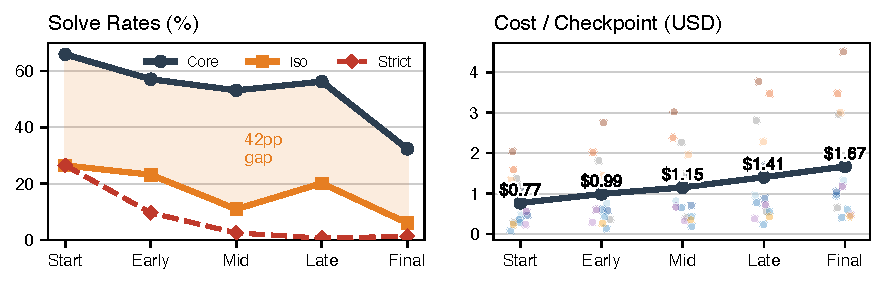
\includegraphics[width=\textwidth]{figures/overview_solve_cost.pdf}
    \caption{\textbf{Performance degrades as problems progress and cost per checkpoint steadily rise.} \emph{Left:} Checkpoint solve rate by type. \emph{Right:} Mean cost per checkpoint as problems progress.}
    \label{fig:solve-cost}
\end{figure}

\autoref{fig:solve-cost} shows the gap between core and isolated pass rates widens from \abFigCoreIsoRatioMin{}$\times$ to \abFigCoreIsoRatioMax{}$\times$. Core pass rate falls from \overallTestCorePassEarlyPct{}\% to \overallTestCorePassLatePct{}\%. Functionality pass rate changes by less than six points, from \overallTestFuncPassEarlyPct{}\% to \overallTestFuncPassLatePct{}\%, while error pass rate drops from \overallTestErrorPassEarlyPct{}\% to \overallTestErrorPassLatePct{}\%.

Cost and context grow while code movement declines. Mean cost per checkpoint grows \abFigCostGrowth{}$\times$ from the start to end, while mean relative lines changed fall from \overallChurnMeanEarlyPct{}\% early to \overallChurnMeanLatePct{}\% late. Total recorded token accounting is \overallTokensTotalB{}B tokens. Normalized to 196 checkpoints, \overallTokenLowestModel{} has the lowest token spend at \overallTokenLowestNormB{}B tokens, while \overallTokenHighestModel{} has the highest at \overallTokenHighestNormB{}B tokens. 
\subsection{Iterative Agent Trajectories Accumulate Quality Issues}\label{sec:iteraitve-degrade}

\begin{figure}[ht]
    \centering
    \makebox[\textwidth][c]{%
        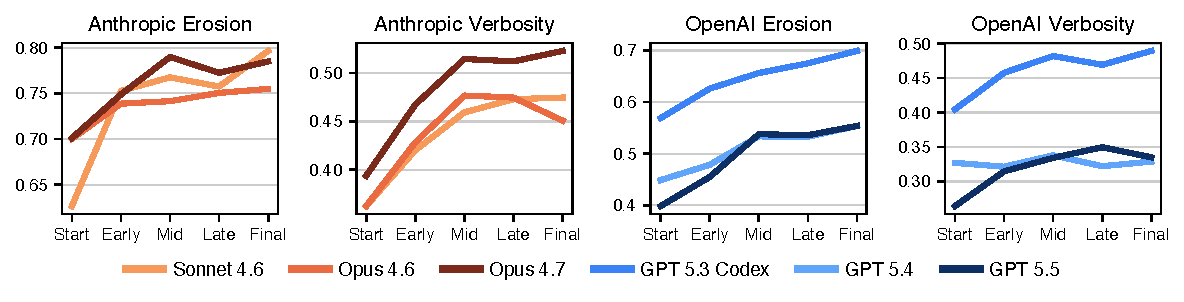
\includegraphics[width=1.15\textwidth]{figures/complexity_sign_flip.pdf}%
    }
    \caption{\textbf{Models from both frontier labs produce similar degradation trends as the problem progresses}. Erosion and verbosity across problem progress for six representative models.}
    \label{fig:accumulation-results}
\end{figure}

\autoref{fig:accumulation-results} highlights the changes in quality throughout frontier models' trajectories on problems. Across all settings, structural erosion increases in \erosionPctIncreasing\% of trajectories, verbosity in \vfTrajIncPct\%. The average number of functions with at least 10 cyclomatic complexity rises from \erosionHighCcCountFirstMean{} to \erosionHighCcCountLastMean{} and mean maximum CC from \newErosionFirstCcMaxMean{} to \newErosionLastCcMaxMean{}. This behavior would be invisible without iterative evaluation.

Opus~4.7's \texttt{main()} on \href{https://www.scbench.ai/problems/forge}{\texttt{forge}} grows \erosionForgeMainCcMultiplier$\times$ in CC across \erosionForgeNumCkpts{} checkpoints, from \erosionForgeMainLinesFirst{} to \erosionForgeMainLinesLast{} lines. The $\ckpt{1}$ \texttt{argparse} call, shown in \autoref{lst:erosion-main-cp1}, is replaced by a manual flag loop in which seven flags each get an identical pair of \verb|--X val|/\verb|--X=val| branches and no helper is extracted (\autoref{lst:erosion-main-cp8}). The accumulation over time highlights the key failure mode.

Verbosity behaves similarly to erosion. Structural duplication grows \vfCloneGrowthPct\% while AST-grep violation density grows only \vfAstOverallGrowth\%, reflecting the rewriting of existing code rather than fresh rule violations. \textbf{Iterative evaluation makes accumulation visible; small structural choices are amplified by iteration rather than absorbed.}

\subsection{How does agent degradation compare to repository histories?}
\label{sec:agent-vs-human}

\begin{figure}[t]
    \centering
    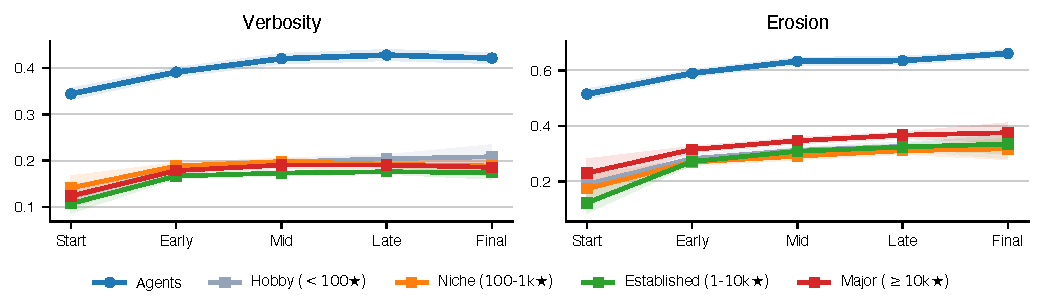
\includegraphics[width=\linewidth]{figures/agent_human_trajectory.pdf}
    \caption{\textbf{Agents produce lower quality code and degrade it faster than real developers.} Verbosity and erosion across normalized trajectory progress, with 95\% confidence intervals. GitHub-star bins over \avhPanelN{} repositories for a total of $\avhTemporalCkpts$ checkpoints. \autoref{tab:agent-vs-human} has HEAD commit details.}
    \label{fig:agent-human-trajectory}
\end{figure}

To answer this, we collect \avhPanelN{} Python repositories ranging from hobby projects under 100 stars to major frameworks with over 10k stars and 2M LOC, covering web frameworks, scientific computing, infrastructure, and utilities. For each repository, we randomly sample up to 30 source-modifying commits totaling \avhTemporalCkpts{} commits. We treat each repository's most recent commit at the time of collection as its current state for cross-sectional comparisons and the full commit sequence as analogous to an agent trajectory.

\autoref{fig:agent-human-trajectory} shows the human panel averages 0.19 verbosity and 0.34 erosion. Agent checkpoints sit \avhAllVerbRatio{}$\times$ and \avhAllErosionRatio{}$\times$ above those means. Only \avhHumanAboveAgentVerbN{} of \avhPanelN{} repositories cross the agent verbosity mean. Agent verbosity grows by \avhAgentVerbSlopeMedian{} per checkpoint and erosion by \avhAgentErosSlopeMedian{}; the human medians are \avhHumanVerbSlopeMedian{} and \avhHumanErosSlopeMedian{}. Inside the iteration loop, agents accumulate verbosity roughly 7$\times$ faster and erosion 5$\times$ faster. Erosion rises in \erosionPctIncreasing{}\% of agent trajectories against \avhTemporalErosRisingPct{}\% of human repositories.

\begin{table}[t]
    \centering
    \caption{Verbosity and erosion at HEAD commit, by GitHub-star tier and against agent checkpoints.}
    \label{tab:agent-vs-human}
    \footnotesize
    \setlength{\tabcolsep}{6pt}
    \begin{tabular}{lccc}
        \toprule
        Group & $n$ & Verbosity & Erosion \\
        \midrule
        Hobby ($< 100\bigstar$) & 114 & $0.21 \pm 0.14$ & $0.33 \pm 0.25$ \\
        Niche ($100\text{--}1\text{k}\bigstar$) & 124 & $0.19 \pm 0.11$ & $0.32 \pm 0.22$ \\
        Established ($1\text{k}\text{--}10\text{k}\bigstar$) & 120 & $0.18 \pm 0.08$ & $0.33 \pm 0.20$ \\
        Major ($\geq 10\text{k}\bigstar$) & 115 & $0.19 \pm 0.10$ & $0.37 \pm 0.19$ \\
        \midrule
        Human panel (all) & 473 & $0.19 \pm 0.11$ & $0.34 \pm 0.22$ \\
        Agent checkpoints & 2869 & $0.44 \pm 0.18$ & $0.68 \pm 0.20$ \\
        \bottomrule
    \end{tabular}
\end{table}


For the \avhAgentEraBothN{} repositories with at least three commits in each of the pre- and post-January-2024 windows, within-repository medians shift by $+\avhAgentEraVerbShiftMedian$ for verbosity and $+\avhAgentEraErosShiftMedian$ for erosion; \avhAgentEraErosHigherPct{}\% of these repositories are more eroded after 2024 than before. The shift is consistent with a small uptick in human-authored slop after agent assistance became common, and it remains far below what an agent accumulates in a single checkpoint. \autoref{sec:human-repo-panel} extends this analysis. 
    
\subsection{Explicit Prompting Improves Initial Quality, But Still Degrades}
\label{sec:prompt-strategy}
We next evaluate whether prompt-side modifications can mitigate the degradation induced by iteration. Two prompts are tested against the \justsolve{}~ baseline. \antislop{} (\autoref{lst:anti-slop-prompt}) enumerates verbosity and over-engineering patterns the agent should avoid. \planfirst{} (\autoref{lst:plan-first-prompt}) requires the agent to produce a written plan before generating code.

\begin{figure}[t]
    \centering
    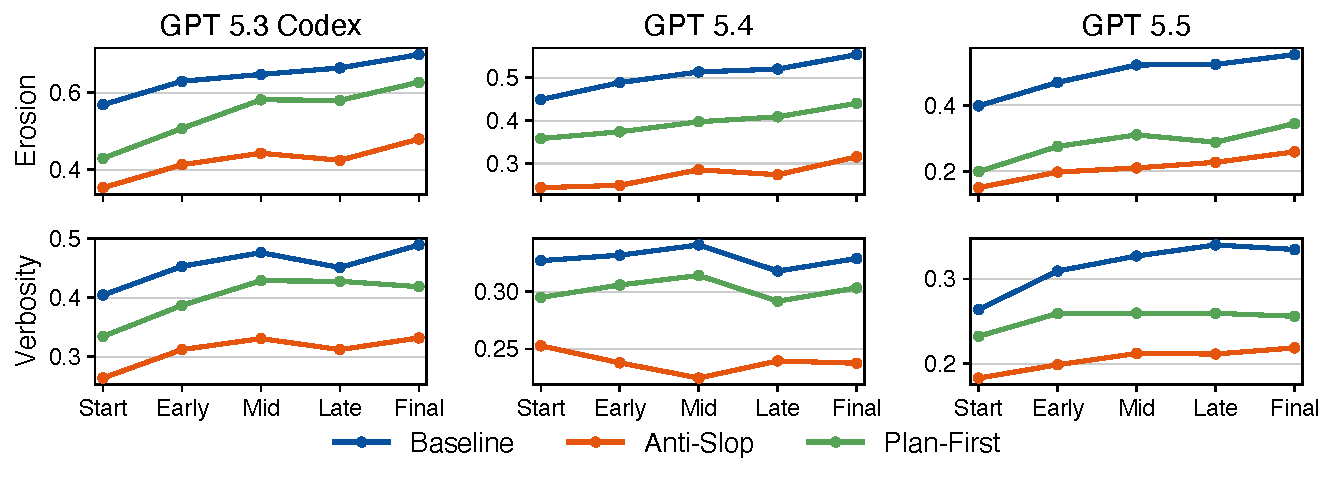
\includegraphics[width=\textwidth]{figures/prompt_strategy_trajectories.pdf}
    \caption{\textbf{Prompting can improve initial quality, but does not remove the iterative issues.} Mean structural erosion (top) and verbosity (bottom) at each progress bin, per model.}
    \label{fig:prompt-strategy-trajectories}
\end{figure}

\definecolor{good}{HTML}{1B7837}
\definecolor{bad}{HTML}{B2182B}
\begin{table}[t]
    \centering
    \caption{Raw values per prompt with the lift over \justsolve{} in parentheses. \textcolor{good}{Green} means improvements while \textcolor{bad}{red} indicates regressions.}
    \label{tab:prompt-strategy-lift}
    \footnotesize
    \setlength{\tabcolsep}{5pt}
    \begin{tabular}{llcccccc}
        \toprule
        Model & Prompt & Strict & Iso. & Core & Erosion & Verbosity & Cost \\
        \midrule
        \multirow{3}{*}{GPT 5.3 Codex} & Just-Solve & 11.2 & 26.0 & 60.7 & 0.64 & 0.46 & 0.66 \\
         & Anti-Slop & 11.2 (+0.0) & 23.5 (\textcolor{bad}{-2.6}) & 57.1 (\textcolor{bad}{-3.6}) & 0.42 (\textcolor{good}{-0.22}) & 0.31 (\textcolor{good}{-0.15}) & 0.73 (\textcolor{bad}{+0.07}) \\
         & Plan-First & 8.2 (\textcolor{bad}{-3.1}) & 21.4 (\textcolor{bad}{-4.6}) & 62.2 (\textcolor{good}{+1.5}) & 0.55 (\textcolor{good}{-0.10}) & 0.40 (\textcolor{good}{-0.06}) & 0.68 (\textcolor{bad}{+0.02}) \\
        \midrule
        \multirow{3}{*}{GPT 5.4} & Just-Solve & 10.7 & 23.5 & 62.8 & 0.51 & 0.33 & 0.72 \\
         & Anti-Slop & 9.2 (\textcolor{bad}{-1.5}) & 25.5 (\textcolor{good}{+2.0}) & 61.2 (\textcolor{bad}{-1.5}) & 0.28 (\textcolor{good}{-0.23}) & 0.24 (\textcolor{good}{-0.09}) & 0.90 (\textcolor{bad}{+0.18}) \\
         & Plan-First & 9.7 (\textcolor{bad}{-1.0}) & 25.0 (\textcolor{good}{+1.5}) & 63.3 (\textcolor{good}{+0.5}) & 0.39 (\textcolor{good}{-0.11}) & 0.30 (\textcolor{good}{-0.02}) & 0.83 (\textcolor{bad}{+0.11}) \\
        \midrule
        \multirow{3}{*}{GPT 5.5} & Just-Solve & 14.8 & 28.1 & 66.8 & 0.49 & 0.32 & 1.51 \\
         & Anti-Slop & 9.2 (\textcolor{bad}{-5.6}) & 24.0 (\textcolor{bad}{-4.1}) & 63.3 (\textcolor{bad}{-3.6}) & 0.21 (\textcolor{good}{-0.28}) & 0.21 (\textcolor{good}{-0.11}) & 1.68 (\textcolor{bad}{+0.17}) \\
         & Plan-First & 8.2 (\textcolor{bad}{-6.6}) & 24.0 (\textcolor{bad}{-4.1}) & 67.3 (\textcolor{good}{+0.5}) & 0.29 (\textcolor{good}{-0.21}) & 0.25 (\textcolor{good}{-0.06}) & 1.61 (\textcolor{bad}{+0.11}) \\
        \bottomrule
    \end{tabular}
\end{table}



\autoref{fig:prompt-strategy-trajectories} highlights that the magnitudes of structural erosion and verbosity are significantly lowered by prompt strategies. Under \antislop{}, verbosity is lower than baseline by \psGptFiveFourAntiSlopVerbPctRed\% on GPT~5.4, \psGptFiveFiveAntiSlopVerbPctRed\% on GPT~5.5, and \psCodexAntiSlopVerbPctRed\% on GPT~5.3~Codex. Erosion is lower by \psGptFiveFourAntiSlopEroPctRed\%, \psGptFiveFiveAntiSlopEroPctRed\%, and \psCodexAntiSlopEroPctRed\% respectively. Only with GPT 5.4 do we observe that quality \emph{improves} from start to end with the \antislop{} prompt.

This improved quality comes with some trade-offs, as highlighted in \autoref{tab:prompt-strategy-lift}. Across models, the base \justsolve~prompt has the best strict performance with an average drop of \psLiftStrictDropAntiSlop~pp for \antislop~and \psLiftStrictDropPlanFirst~pp for \planfirst. Core pass rate improves by 0.8~pp for \planfirst. Both prompts raise the cost per checkpoint by \psLiftCostIncreasePct\% on average. \textbf{Overall, prompting strategies trade capabilities for better initial quality, with little impact on the iterative degradation.}
